% CMS UK Talk 2011 (Bristol)
\documentclass{beamer}
\usetheme{iclpt}
\begin{document}

\title{Fitting SUSY Parameters and Early CMS Results}
\author{Sam Rogerson}
\institute{Imperial College London}
\date{\today}

\begin{frame}[plain]
\titlepage
\end{frame}

\begin{frame}{Outline}
\tableofcontents
\end{frame}


%%%%%%%%%%%%%%%%%%%%%%%%%%%%%%%%%%%%%%%%%%%%%%%%%%%%%%%%%%%%%%%%%%%%%%%%%%%%%%%
% Introduction
%---------------------------------
\begin{frame}{Aims}
\section{\insertframetitle}
  \begin{itemize}
    \item Explore the parameter spaces of models of supersymmetry (SUSY) to
    understand their features
    \item Determine how consistent particular models of SUSY are with our
    observation
    \item If we do see SUSY, what should it look like? 
    \item If we don't, where might we expect to see it?
  \end{itemize} 
\end{frame}

\begin{frame}{Models Covered}
\section{\insertframetitle}
  \begin{tabular}{ l l l }
    & & \textcolor{gray}{Boundary Conditions}\\
    \alert{CMSSM}  & $m_{0},m_{1/2},A_{0},tan(\beta),\textrm{sign}(\mu)$  & 
    \textcolor{gray}{Unification + } \\ \\ 
    VCMSSM & $m_{0},m_{1/2},A_{0},\textrm{sign}(\mu)$ & $B_{0}=A_{0}+m_{0}$  \\
    \\
    \alert{MSUGRA} & $m_{0},m_{1/2},A_{0},\textrm{sign}(\mu)$ & $B_{0}=A_{0}+m_{0};
    m_{0}=m_{3/2}$  \\ \\
    NUHM1  & $m_{0},m_{1/2},A_{0},m_{1,2}^{2},\textrm{sign}(\mu)$ & $m_{1,2} =
    m_{0} + \Delta m_{H}$  \\ \\
  \end{tabular}
\end{frame}

\begin{frame}{Observables}
\section{\insertframetitle}
  \textcolor{gray}{Examples}
  \begin{columns}[t]
  \column{2.0in}
  \begin{itemize}
    \item Flavour Physics 
      \begin{itemize}
        \item $\textrm{R}\left(b\rightarrow s\gamma\right)$
        \item $\textrm{BR}\left(B_{s}\rightarrow\mu\mu\right)$
        \item $\textrm{R}\left(B\rightarrow\tau\nu\right)$
      \end{itemize}
    \item EWPOs 
      \begin{itemize}
        \item $\Gamma_{Z}$
        \item $\textrm{A}_{fb}(b)$,$\textrm{A}_{fb}(c)$
      \end{itemize}
  \end{itemize}
  \column{2.0in}
  \begin{itemize}
    \item Cosmology
      \begin{itemize}
        \item $\Omega h^{2}$ 
        \item $\sigma_{p}^{SI}$
      \end{itemize}
    \item Particle Spectrum
      \begin{itemize}
        \item $M_{h^{0}}$ of particular interest
      \end{itemize}
    \item Other indirect constraints
      \begin{itemize}
        \item $\Delta(g_{\mu}-2)$
      \end{itemize}
  \end{itemize}
  \end{columns}

\end{frame}

\begin{frame}{Global Likelihood Function}
\section{\insertframetitle}
\begin{eqnarray}
  \chi^{2}=&\sum_{i}^{N}\frac{\left(C_{i}-P_{i}\right)^2}{\sigma\left(C_{i}\right)^2+\sigma\left(P_{i}\right)^2}\\
	  +&\chi^{2}\left(M_{h}\right)+\chi^{2}\left(\textrm{BR}\left(B_{s}\rightarrow\mu\mu\right)\right)\\
	  +&\chi^{2}\left(\textrm{SUSY search limits}\right)\\
	  +&\sum_{i}^{M}\frac{\left(f_{SM_{i}}^{\textrm{obs}}-f_{SM_{i}}^{\textrm{fit}}\right)^{2}}{\sigma\left(f_{SM_{i}}\right)^{2}}\\
    +&\alert{\chi^{2}(\hdots)}
\end{eqnarray}
\end{frame}

\begin{frame}{CMS Constraint}
\section{\insertframetitle}
  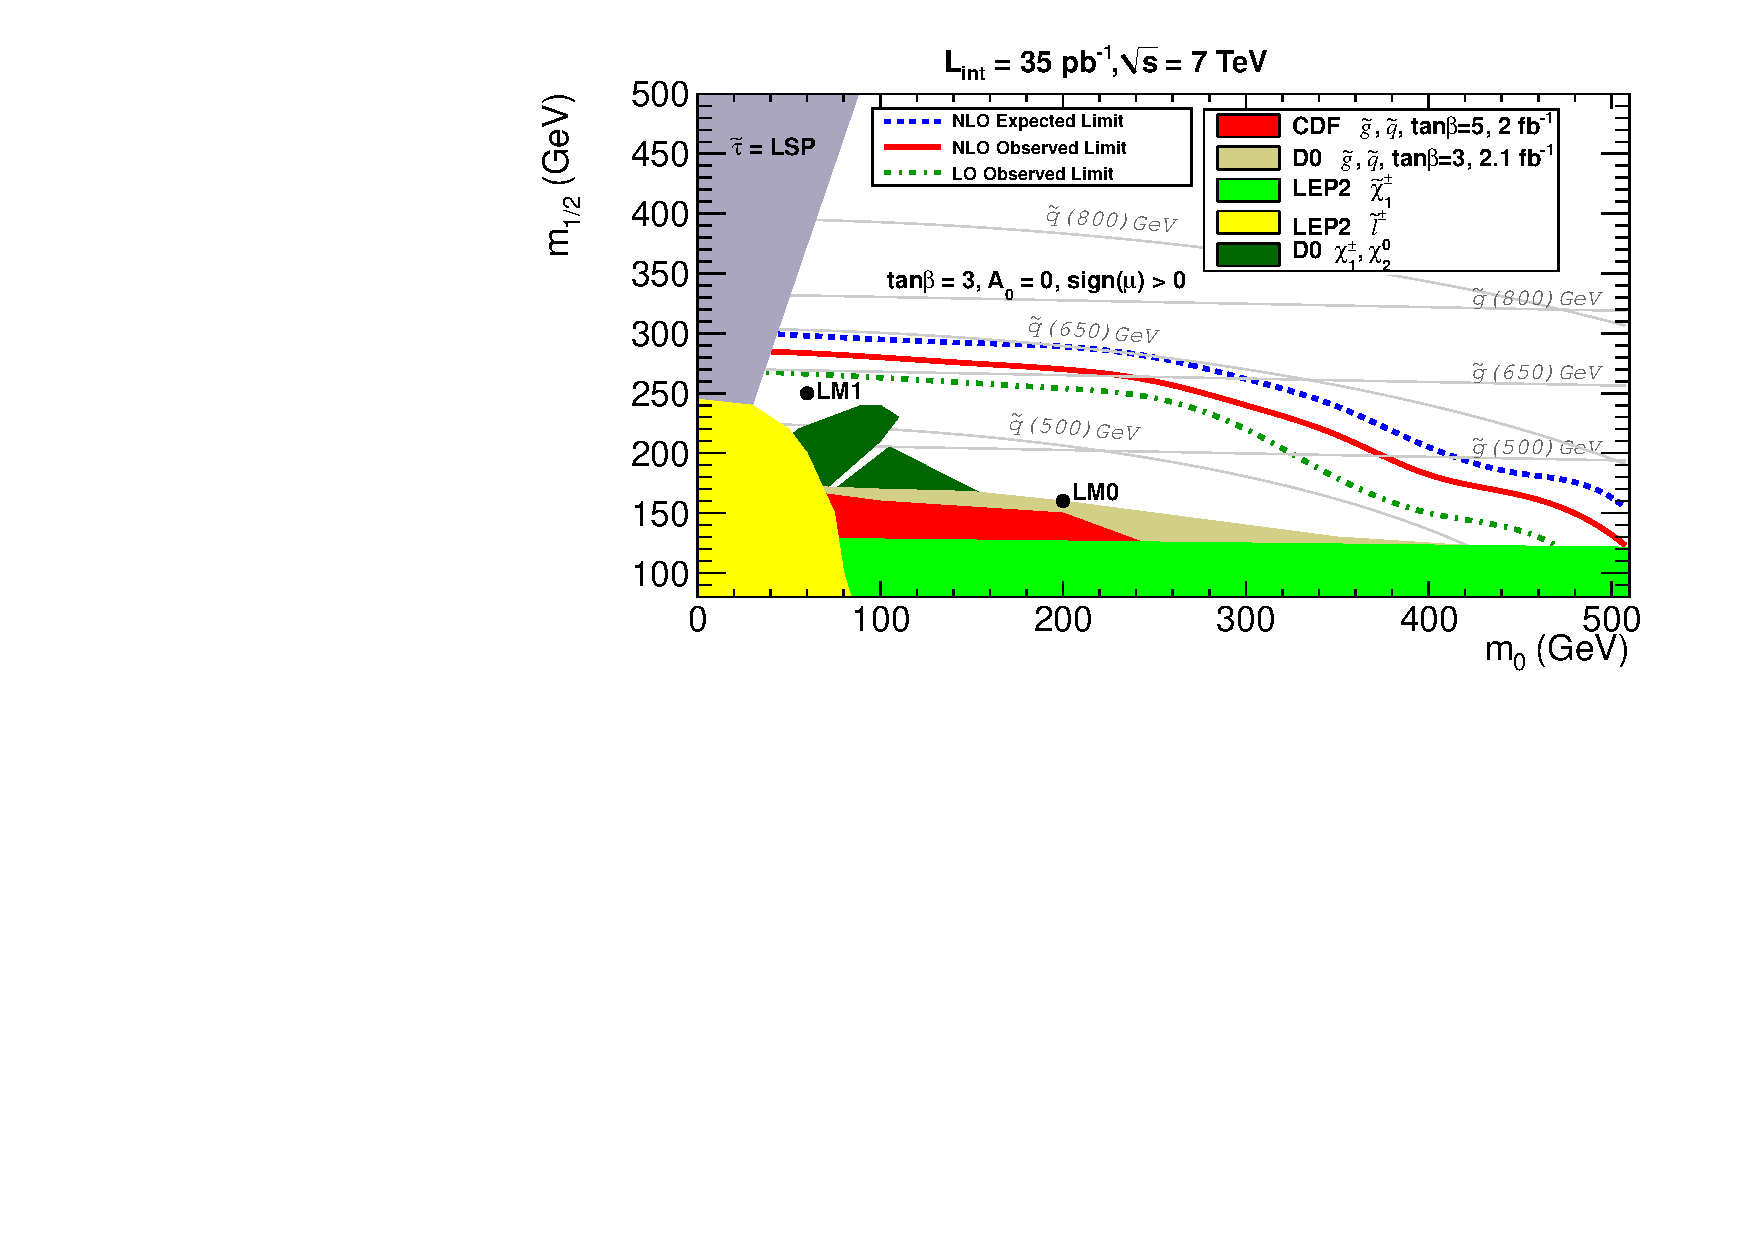
\includegraphics[height=5cm]{cms-excl.pdf}
\end{frame}

\begin{frame}{CMS Constraint: Function}
\section{\insertframetitle}
  \begin{columns}[]
    \column{1.7in}
    \begin{eqnarray*}
      \chi^{2}_{CMS} = \chi^{2}_{\infty}\left|\frac{M_{C}}{M} - 1\right|^{P}, \\
      M\equiv \left(m_{0}^{2}+m_{1/2}^{2}\right)^{1/2}
    \end{eqnarray*}
    \begin{itemize}
      \item $\displaystyle\lim_{M\rightarrow\infty}\chi^{2}_{CMS}=\chi^{2}_{\infty}$
      \item $\chi^{2}_{CMS}\displaystyle({M=M_{C}}) = 0$
    \end{itemize}
    \column{2.0in}
    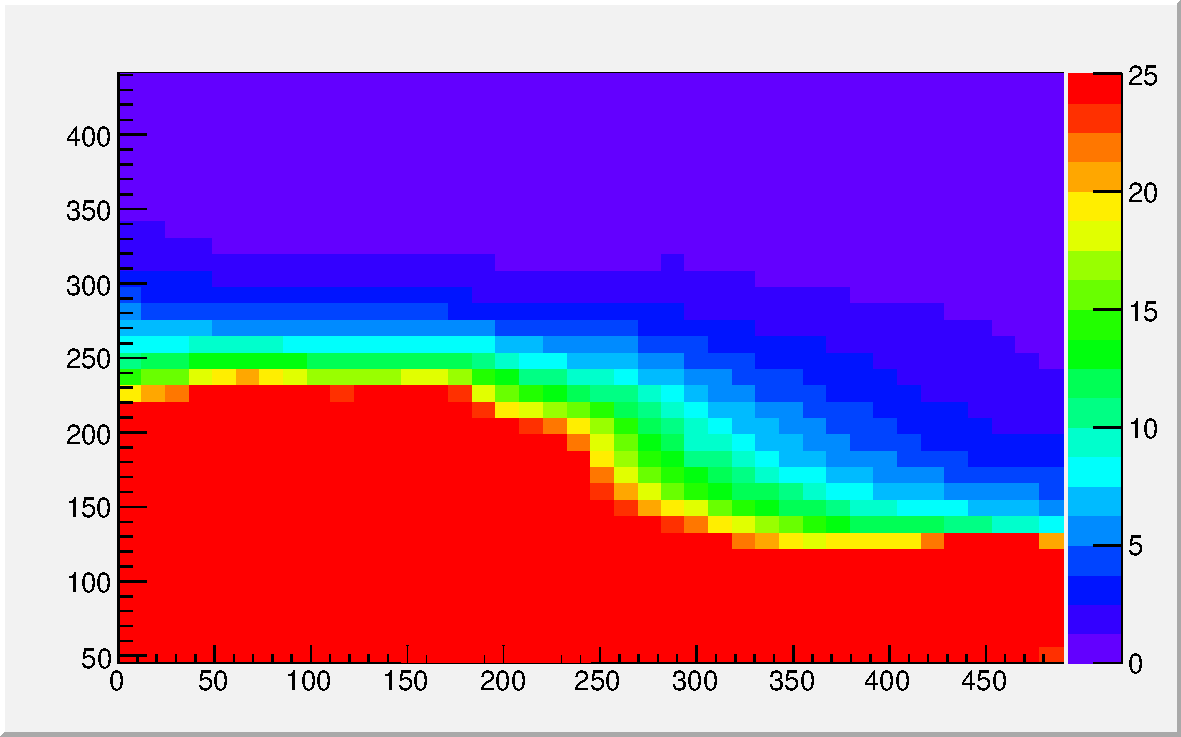
\includegraphics[height=3.5cm]{cms-lfunc.pdf}
  \end{columns}
\end{frame}

\begin{frame}{CMS Constraint: Parameter values}
\section{\insertframetitle}
\begin{columns}[t]
  \column{2.0in}
$\chi^{2}_{\infty}$
  \begin{itemize}
    \item Observed events $= 13$
    \item $\textrm{SM}_{bkg}=10.5^{+3.6}_{-2.5}$
    \item Excess$ = 2.5$
    \item $95\% CL$: number of signal events compatible with the
    excess $ = 13.4$ ($95\%=1.96\sigma$)
    \item Total numbr of events for any signal $=2.5\pm5.56$
    \item \emph{$\chi^{2}_{\infty}=0.85$}
  \end{itemize}
  \column{2.0in}
  NLO Expected (absense):
  \begin{itemize}
    \item 10.9 events
    \item $(10.9-2.5)/5.56\Rightarrow 1.51\sigma$
    \item \emph{$\chi^{2}_{NLO_{e}} = 4.06$}
  \end{itemize}
  NLO Observed:
  \begin{itemize}
    \item Similarly, $95\%=1.96\sigma\Rightarrow\alert{\chi^{2}_{NLO_{o}}=
    5.99}$ 
  \end{itemize}
  \it{These are used as boundary condition on our function}

\end{columns}
\end{frame}


\end{document}
